\section{PatchMatch Stereo}

传统的双目立体匹配计算视差时往往通过均值滤波取得某个点的视差,而
\textbf{PatchMatch Stereo - Stereo Matching with Slanted Support Windows}\protect
\footnote{\url{https://projet.liris.cnrs.fr/imagine/pub/proceedings/BMVC-2011/Paper_289/PatchMatchStereo_ExtentedAbstract.pdf}}构建LR过程,将邻居点及视差匹配的其他视图的点作为样本,学习LR对应的三个参数,因此效果好于传统均值滤波。

\subsection{双目立体匹配}

\begin{figure}[H]
	\begin{center}
		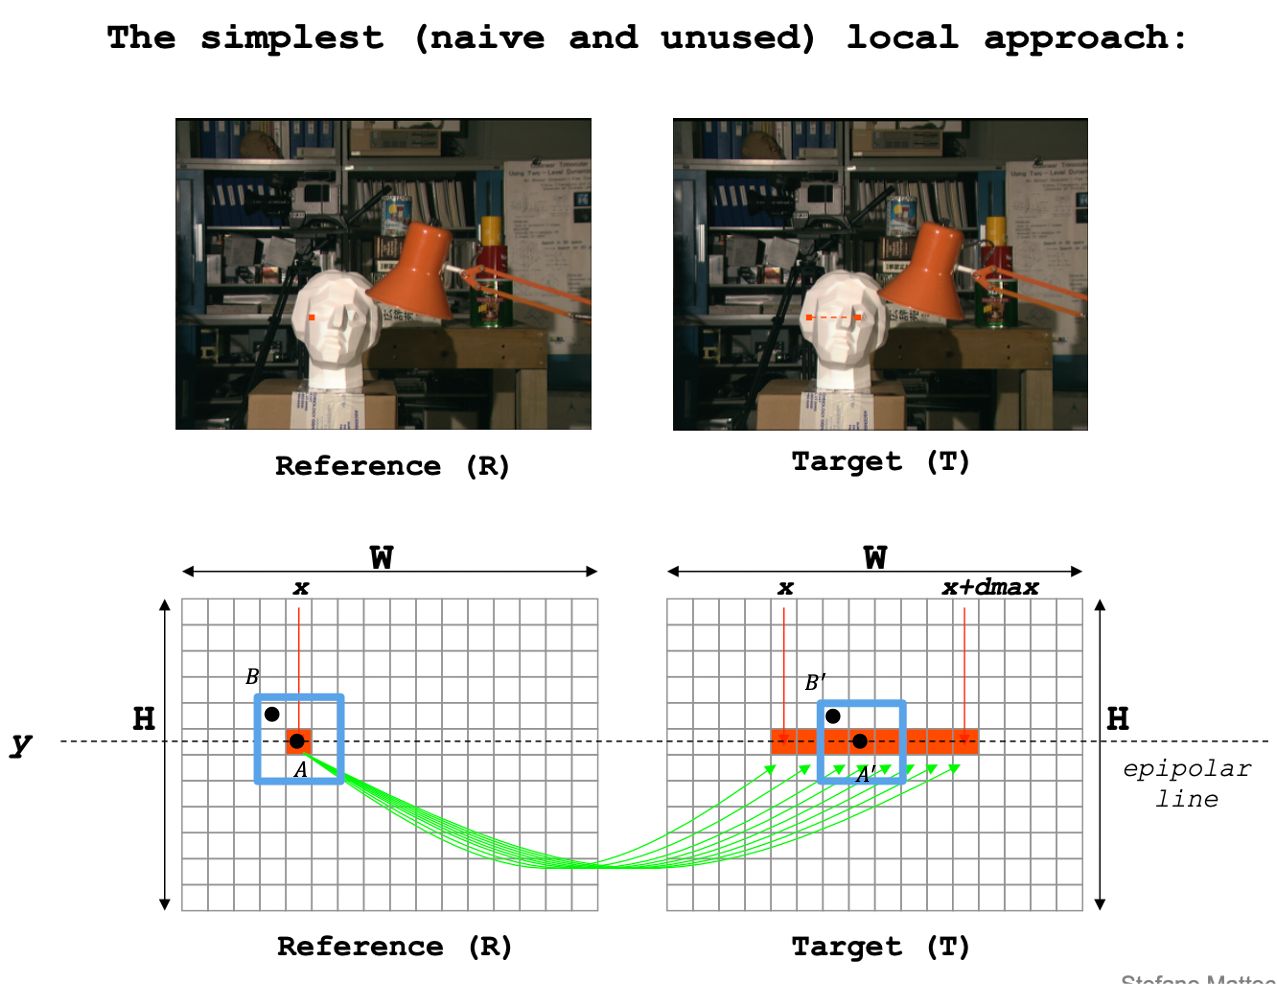
\includegraphics[width=\textwidth]{../images/disparty_constrain.png}
	\end{center}
	\caption{沿扫描线(极线)寻找匹配点}
\end{figure}

传统的双目立体匹配,沿着扫描线寻找某个点的最佳匹配,包括4个步骤,
\begin{enumerate}
	\item 代价计算,衡量两张图像上点对的匹配代价,代价可通过两点灰度绝对值差、绝对值和、归一化相关系数、互信息、Census变换、Rank变换等方法衡量
	\item 代价聚合,为降低单点对匹配带来的噪音,通过局部或者全局的方式优化匹配代价
		\begin{itemize}
			\item 局部方法,在\textit{支撑窗口}做均值滤波,又分为\textit{固定窗}和\textit{自适应窗}
			\item 全局方法,定义一能量函数,最小化整体点点代价匹配,转化为一个优化问题
		\end{itemize}
	\item 视差计算,取代价最小的视差作为真值
	\item 视差优化,手段包括提高精度,比如上图通过二次曲线拟合将视差整数值扩展到浮点值;剔除错误匹配、弱纹理优化、填补空洞等
\end{enumerate}

在代价计算和代价聚合的局部方法都可以借助一个窗口进行局部计算,代价聚合阶段的窗口命名为\textit{\textbf{support window}},主要操作便是在在窗口内对代价进行均值滤波。\\

通过上图可知,对应窗口内所有点对的视差都是相同的,比如$(A,A^\prime),(B,B^\prime)$,因为它们的视差偏移量是相同的。\\

因此,支持窗口本身隐含了窗口内的视差是个常量,或者说即深度是个常量,这显然是不合理的,文中开篇便给出反例,
\begin{itemize}
	\item $A,B$在不同的曲面上
	\item $A,B$处在斜面上
\end{itemize}

反之当$A,B$具有不同深度的时候,也具有不同的视差,如果$(A,A^\prime)$是对应点对,那$(B,B^\prime)$不应该是对应点对,此时$(B,B^\prime)$的匹配代价会很高,会给基于窗口的均值操作会给代价聚合带来很高的的误差。

\subsection{PatchMatch Stereo算法}

作者认为,窗内点在不同曲面的问题,可通过\textit{自适应窗口}解决,并且有很多解决方案;但点在斜面的问题关注的并不多,因此他提出\textit{slanted support window}来应该对该问题。\\

那么,$A,B$在不同的曲面上与在相同斜面上有什么本质区别呢?我个人认为,区别是深度值的变化是否连续,斜面上点的深度变化连续,而不同曲面则不连续。\\

不连续值通过RGB差异便可区分,因为不同深度的点,RGB不同的概率是很大的,所以作者说通过自适应窗口来解决;相反,连续值的RGB变化不明显,通过权重自适应的方法便不再有效。\\

前面提到,\textit{support window}假设内部所有点的视差相同,\textit{slanted support window}则放开次约束;二者都是一个$w\times h$的2D像素窗口,区别就是每点视差是否相同。\\

在基于流形的建模场景,会沿着场景表面构建局部邻域进行计算,比如人脸识别中的球面卷积,这种局部邻域不再是2D窗口。\textit{slanted support window}未拟合表面几何,仅在2D窗口中赋以不同的视差度量方式。\\

\textit{slanted support window}中点的视差是通过评估\textit{视差平面}确定,视差变化是连续的,所以对应的视差平面最优解一定存在。

\begin{figure}[H]
	\begin{center}
		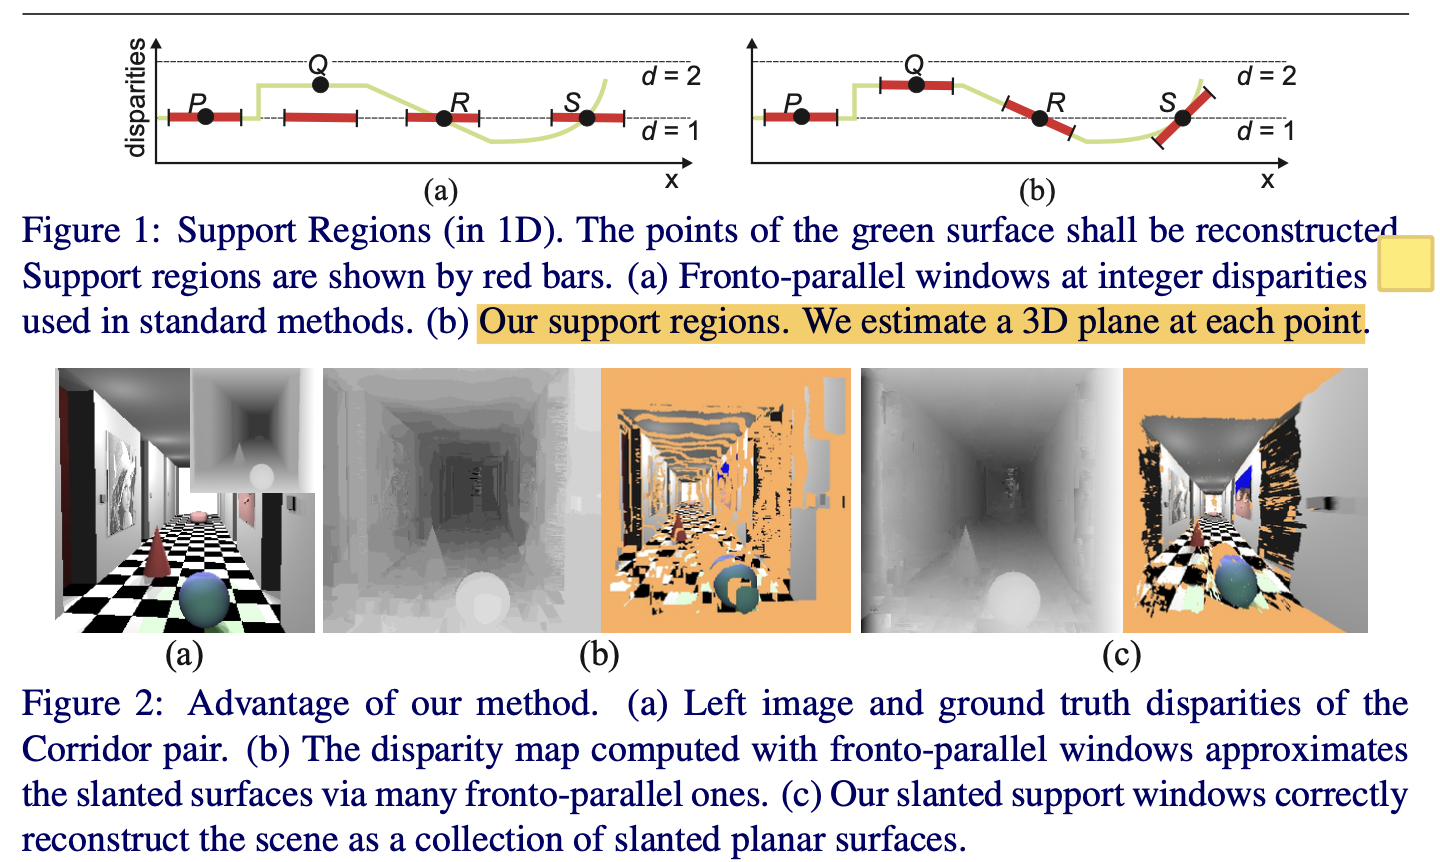
\includegraphics[width=\textwidth]{../images/slanted_window.png}
	\end{center}
\end{figure}

图(a)是\textit{support window},窗口内所有点的视差值都相同;图(b)是\textit{slanted support window},每个点的视差不同。

\subsubsection*{视差平面建模}

$f_p$为$p$点对应的视差平面,$\mathbf{n}_p = (a_{f_p}, b_{f_p}, c_{f_p})^T$为$f_p$的法向量,文中给出$p$点视差计算公式,

\begin{equation}
	d_p = a_{f_p}p_x + b_{f_p}p_y+c_{f_p}\label{disparity_eq}
\end{equation}

只有两个变量$p_x,p_y$,怎么看都不是一个平面方程,这实际是像素平面上的直线方程,投影回三维空间才能看出等价的平面方程,具体操作如下:\\

上式用齐次坐标及内积表示为,

$$
	d_p = \mathbf{p}^T\cdot \mathbf{n}_p
$$

$\mathbf{p}=(p_x,p_y,1)^T$为$p$的二维齐次坐标,相机内参矩阵为$\mathbf{K}$,$P = \mathbf{K}^{-1}\mathbf{p}$为$p$的3D坐标,

\begin{align*}
		d_p &= \left(\mathbf{K}\mathbf{K}^{-1}\mathbf{p}\right)^T\cdot \mathbf{n}_p \\
			&= P^T\cdot \left(\mathbf{K}^T \mathbf{n}_p\right)\\
			&\overset{\triangle}{=}P^T\cdot \mathbf{n}_p
\end{align*}

因为$\mathbf{K}$是常量,$\mathbf{n}_p$是需学习参数,所以$\mathbf{K}^T \mathbf{n}_p$仍用$\mathbf{n}_p$表示。\\

整理一下可得,
$$
	\mathbf{n}_p^T P =d_p
$$

这才是$p$点的\textbf{\textit{视差平面}}方程,$f_p = (a_f,b_f,c_f,-d_p)^T$,视差$d_p$是该平面的截距。

\subsubsection*{视差平面计算}

视差平面过$P$点,所以只要确定法向量$\mathbf{n}_p$,平面便可被唯一确定,文中给出如下优化目标,

\begin{equation}
	f_p = \underset{f\in \mathcal{F}}{\arg\min} \mathop{m}(p,f)\label{disparity_eq_opt}
\end{equation}

$\mathcal{F}$是平面全集,

\begin{align*}
	\mathop{m}(p,f) &= \sum_{q\in W_p} w(p,q)\cdot \rho\left(q,q-(a_{f}q_x + b_fq_y +c_f)\right) \\
	&= \sum_{q\in W_p} w(p,q)\cdot \rho\left(q,q-d_q\right)\\
	&= \sum_{q\in W_p} w(p,q)\cdot \rho\left(q,q^\prime\right)
\end{align*}

这就是反复提到的在支持窗内对代价做均值,以提升单点代价匹配的抗噪性。\\

$W_p$为$p$点的\textbf{support window},$q^\prime$为$q$在目标图像上的对应点(二者通过视差平移),$w(p,q)$为自适应相似度权重,
$$
	w(p,q) = e^{-\frac{\Vert I_p - I_q\Vert}{\gamma}}
$$

$I_p,I_q$为RGB值,$\gamma$为超参数;

$$
	\rho(q,q^\prime) = (1-\alpha)\cdot \min\left(\Vert I_p - I_q\Vert, \tau_{col}\right) + \alpha\cdot\min\left(\Vert\nabla I_q - \nabla I_{q^\prime} \Vert, \tau_{grad}\right)
$$

为点对匹配代价,通过RGB和梯度相似度来定义,$\mathop{m}(p,f)$则为支持窗内的加权匹配代价。\\

权重$w(p,q)$是一个自适应常数,与优化目标无关,所以优化的主要工作是最小化$q$与$q^\prime$之间的匹配代价,只要每个点的视差达到最优值,则匹配代价也会达到最小,这转变为线性回归问题。\\

此时若有标注样本,简单训练便可得到三个参数。样本是没有的,作者通过一些启发式规则迭代求解上面3个参数。

\subsubsection*{视差平面求解}
	作者给出一些启发规则,及迭代步骤,
	\begin{enumerate}
		\item \textbf{Random Initialization} 
			\begin{itemize}
				\item 随机初始化法向量,但不是直接随机取值,先取值一个视差范围内的$z_0$,对$p=(x_0,y_0)$,构成一个新坐标$P=(x_0,y_0,z_0)$;
				\item 随机初始化单位法向量$\overset{\rightarrow}{\mathbf{n}} = (n_x,n_y,n_z)$,并计算
				$$
					a_f := -\frac{n_x}{n_z}, b_f := -\frac{n_y}{n_z}, c_f := -a_fx_0-b_fy_0+z_0
				$$
			\end{itemize}
			前两步操作有点像齐次坐标转为二维坐标的意思,最后一步是方程(\ref{disparity_eq})。\\

			$(x_0,y_0,z_0)$是在二维坐标$(x_0,y_0)$后面加了$z_0$,是没有意义的坐标,正确的作法是通过$\mathbf{K}^{-1}$反投影$(x_0,y_0,z_0,1)$,再乘以尺度因子$z_0$
		\item \textbf{Iteration} 主要进行下面几个传播过程,主要是寻找使得cost降低的$\mathbf{n}_p$
			\begin{itemize}
				\item \textbf{邻域内(Spatial Propagation)} 检查$p$领域内的$q$点确定的参数,能否使的$p$点的cost降低,如果可以,则采用$q$点的参数,即
				$$
					m(p,f_q) < m(p,f_p)
				$$
				则更新$f_p:=f_q$,可以把$q$看做样本,就是一个单点训练过程。

				\item \textbf{对应图(View Propagation)} 这一步是应用两视图约束,如果右视图上$p$的对应点$p^\prime$的cost更低,则采用这组参数,相比第一步,相当于样本扩展到其他视图。

				\item \textbf{固定位置(Temporal Propagation)} 这是对视频帧而言,不同帧相同位置做类似替换

				\item \textbf{扰动方向(Plane Refinement)} 进一步调整参数,包括两部分,
					\begin{itemize}
						\item 扰动深度,根据实际场景对$z_0$估计一个区间$[-\Delta_{z_0}^{max}, \Delta_{z_0}^{max}]$,构造新点$P^\prime=(x_0,y_0,z_0^\prime)$

						\item 扰动法向,对法向量也做类似限制$[-\Delta_{n}^{max}, \Delta_{n}^{max}]$

						\item 迭代这个过程,看新参数是否使的cost降低;每迭代一次,区间长度折半
					\end{itemize}
			\end{itemize}

			上面几个步骤迭代时顺序执行,且偶数次正序执行,从左上到右下,奇数次反序执行,后续有很多工作使得这个过程可以并行。

		\item \textbf{后处理},根据新参数生成的视差看是否满足左右约束,$|d_p - d_{p^\prime}| <1$,如果不满足,则找附近点的视差代替

	\end{enumerate}

\textit{客观上不存在视差平面,本质上作者定义了一个三参数线性回归拟合每个点的视差;而三维空间的三个参数跟平面一一对应,如此便有了视差平面这一概念;若不是三参数回归或用其他优化方法,就没这样的可解释性。}

\subsection{PatchMatch}

\textbf{PatchMatch: A Randomized Correspondence Algorithm for Structural Image Editing}\protect\footnote{\url{https://gfx.cs.princeton.edu/pubs/Barnes_2009_PAR/patchmatch.pdf}}\\

这是本文经常被提起的一篇文章,实际就是从两张图像中找相似patch,文中提出两个步骤:
\begin{enumerate}
	\item \textbf{Propgation} 如果某两个patch相似,则查找其左侧和下侧的patch
	\item \textbf{Random Search} 如果某个patch相似,则小幅扰动坐标再查找一次
\end{enumerate}

这相比纯粹的随机搜索多了一些策略,计算性能也大幅提升;理论基础是图像是连续的,某个patch相似,则周边也可能相似。\\

PatchMatch Stereo借助了PatchMatch的思想,传播过程比PatchMatch多了几个阶段,随机搜索过程则主要体现在后处理对法向和深度的扰动上。